\documentclass[onecolumn,10pt]{jhwhw}

\usepackage{epsfig} %% for loading postscript figures
\usepackage{amsmath}
\usepackage{graphicx}
\usepackage{grffile}
\usepackage{pdfpages}
\usepackage{algpseudocode}
\usepackage{wrapfig}
\usepackage{pgfplots}
\usepackage{amsfonts}
\usepackage{booktabs}
\usepackage{siunitx}
\usepackage{commath}
\usepackage{rotating}
\usepackage{url}

% Default fixed font does not support bold face
\DeclareFixedFont{\ttb}{T1}{txtt}{bx}{n}{12} % for bold
\DeclareFixedFont{\ttm}{T1}{txtt}{m}{n}{12}  % for normal

% Custom colors
\usepackage{color}
\usepackage{listings}
\usepackage{framed}
\usepackage{caption}
\usepackage{bm}
\captionsetup[lstlisting]{font={small,tt}}

\definecolor{mygreen}{rgb}{0,0.6,0}
\definecolor{mygray}{rgb}{0.5,0.5,0.5}
\definecolor{mymauve}{rgb}{0.58,0,0.82}

\lstset{ %
  backgroundcolor=\color{white},   % choose the background color; you must add \usepackage{color} or \usepackage{xcolor}
  basicstyle=\ttfamily\footnotesize, % the size of the fonts that are used for the code
  breakatwhitespace=false,         % sets if automatic breaks should only happen at whitespace
  breaklines=true,                 % sets automatic line breaking
  captionpos=b,                    % sets the caption-position to bottom
  commentstyle=\color{mygreen},    % comment style
  deletekeywords={...},            % if you want to delete keywords from the given language
  escapeinside={\%*}{*)},          % if you want to add LaTeX within your code
  extendedchars=true,              % lets you use non-ASCII characters; for 8-bits encodings only, does not work with UTF-8
  frame=single,                    % adds a frame around the code
  keepspaces=true,                 % keeps spaces in text, useful for keeping indentation of code (possibly needs columns=flexible)
  columns=flexible,
  keywordstyle=\color{blue},       % keyword style
  language=Python,                 % the language of the code
  morekeywords={*,...},            % if you want to add more keywords to the set
  numbers=left,                    % where to put the line-numbers; possible values are (none, left, right)
  numbersep=5pt,                   % how far the line-numbers are from the code
  numberstyle=\tiny\color{mygray}, % the style that is used for the line-numbers
  rulecolor=\color{black},         % if not set, the frame-color may be changed on line-breaks within not-black text (e.g. comments (green here))
  showspaces=false,                % show spaces everywhere adding particular underscores; it overrides 'showstringspaces'
  showstringspaces=false,          % underline spaces within strings only
  showtabs=false,                  % show tabs within strings adding particular underscores
  stepnumber=1,                    % the step between two line-numbers. If it's 1, each line will be numbered
  stringstyle=\color{mymauve},     % string literal style
  tabsize=4,                       % sets default tabsize to 2 spaces
}

\author{John Karasinski}
\title{Homework 2}

\begin{document}
%\maketitle

\problem{Trapped Particle Radiation}
Assume two spacecraft orbit Earth, one at an altitude of 3000km, the other at 20,000km.
\part{Remind yourself --- are these orbits above or below geostationary?}

\begin{quote}
A geostationary orbit (GEO) is a circular geosynchronous orbit in the plane of the Earth's equator with a radius of approximately 42,164 km (measured from the center of the Earth). A satellite in such an orbit is at an altitude of approximately 35,786 km above mean sea level\footnote{\url{https://en.wikipedia.org/wiki/Geosynchronous_orbit}}.
\end{quote}

\noindent As such, both of these satellites are below geostationary.

\part{Assuming they are both shielded with 4mm aluminum and have the same electronics, which spacecraft is more likely to suffer Single-Event Upsets? Why?}
\\
\\
\indent The most likely place for a satellite to experience a Single-Event Upset is within the Van Allen radiation belts, and one of the safest regions for satellites to be is within the inner and out belt. The inner belt extends from 1,000 to 6,000 kilometers above the Earth, and the outer belt extends from 13,000 to 60,000 kilometers above the Earth's surface.

The inner belt contains high concentrations of electrons in the range of hundreds of keV and energetic protons with energies exceeding 100 MeV, trapped by the relatively strong magnetic fields in the region\footnote{Gusev, A. A.; Pugacheva, G. I.; Jayanthi, U. B.; Schuch, N. (2003). ``Modeling of Low-altitude Quasi-trapped Proton Fluxes at the Equatorial Inner Magnetosphere''. Brazilian Journal of Physics 33 (4): 775–781. Bibcode:2003BrJPh..33..775G.}. Due to this large flux, the satellite in the 3,000km altitude would be more likely to suffer Single-Event Upsets.

\problem{Upper Atmosphere Physics}
\part{What is the change in density of the exosphere at Hubble Space Telescope (HST) altitude between the date of its fourth Shuttle re-boost (Servicing Mission 3B) and the date of your new spacecraft’s re-boost?}

The HST is currently orbiting with a Perigee 551.4 km and an Apogee of 555.6 km\footnote{``HST Satellite details 1990-037B NORAD 20580''. N2YO. January 27, 2015. Retrieved January 27, 2015.}. Servicing Mission 3B took place in March 2002\footnote{https://en.wikipedia.org/wiki/STS-109}, which was during a solar maximum (see Figure~\ref{fig:density}). The date of our proposed mission is January 2020, and the next solar cycle is expected to be ``one of the weakest in centures''\footnote{\url{http://science.nasa.gov/science-news/science-at-nasa/2006/10may_longrange/}}, and should peak around 2022. While it's impossible to know what the density of the exosphere will be in 2020, we should expect the density to be 50\% to 100\% of what is was during Servicing Mission 3B.

\begin{figure}[tb!]
\begin{center}
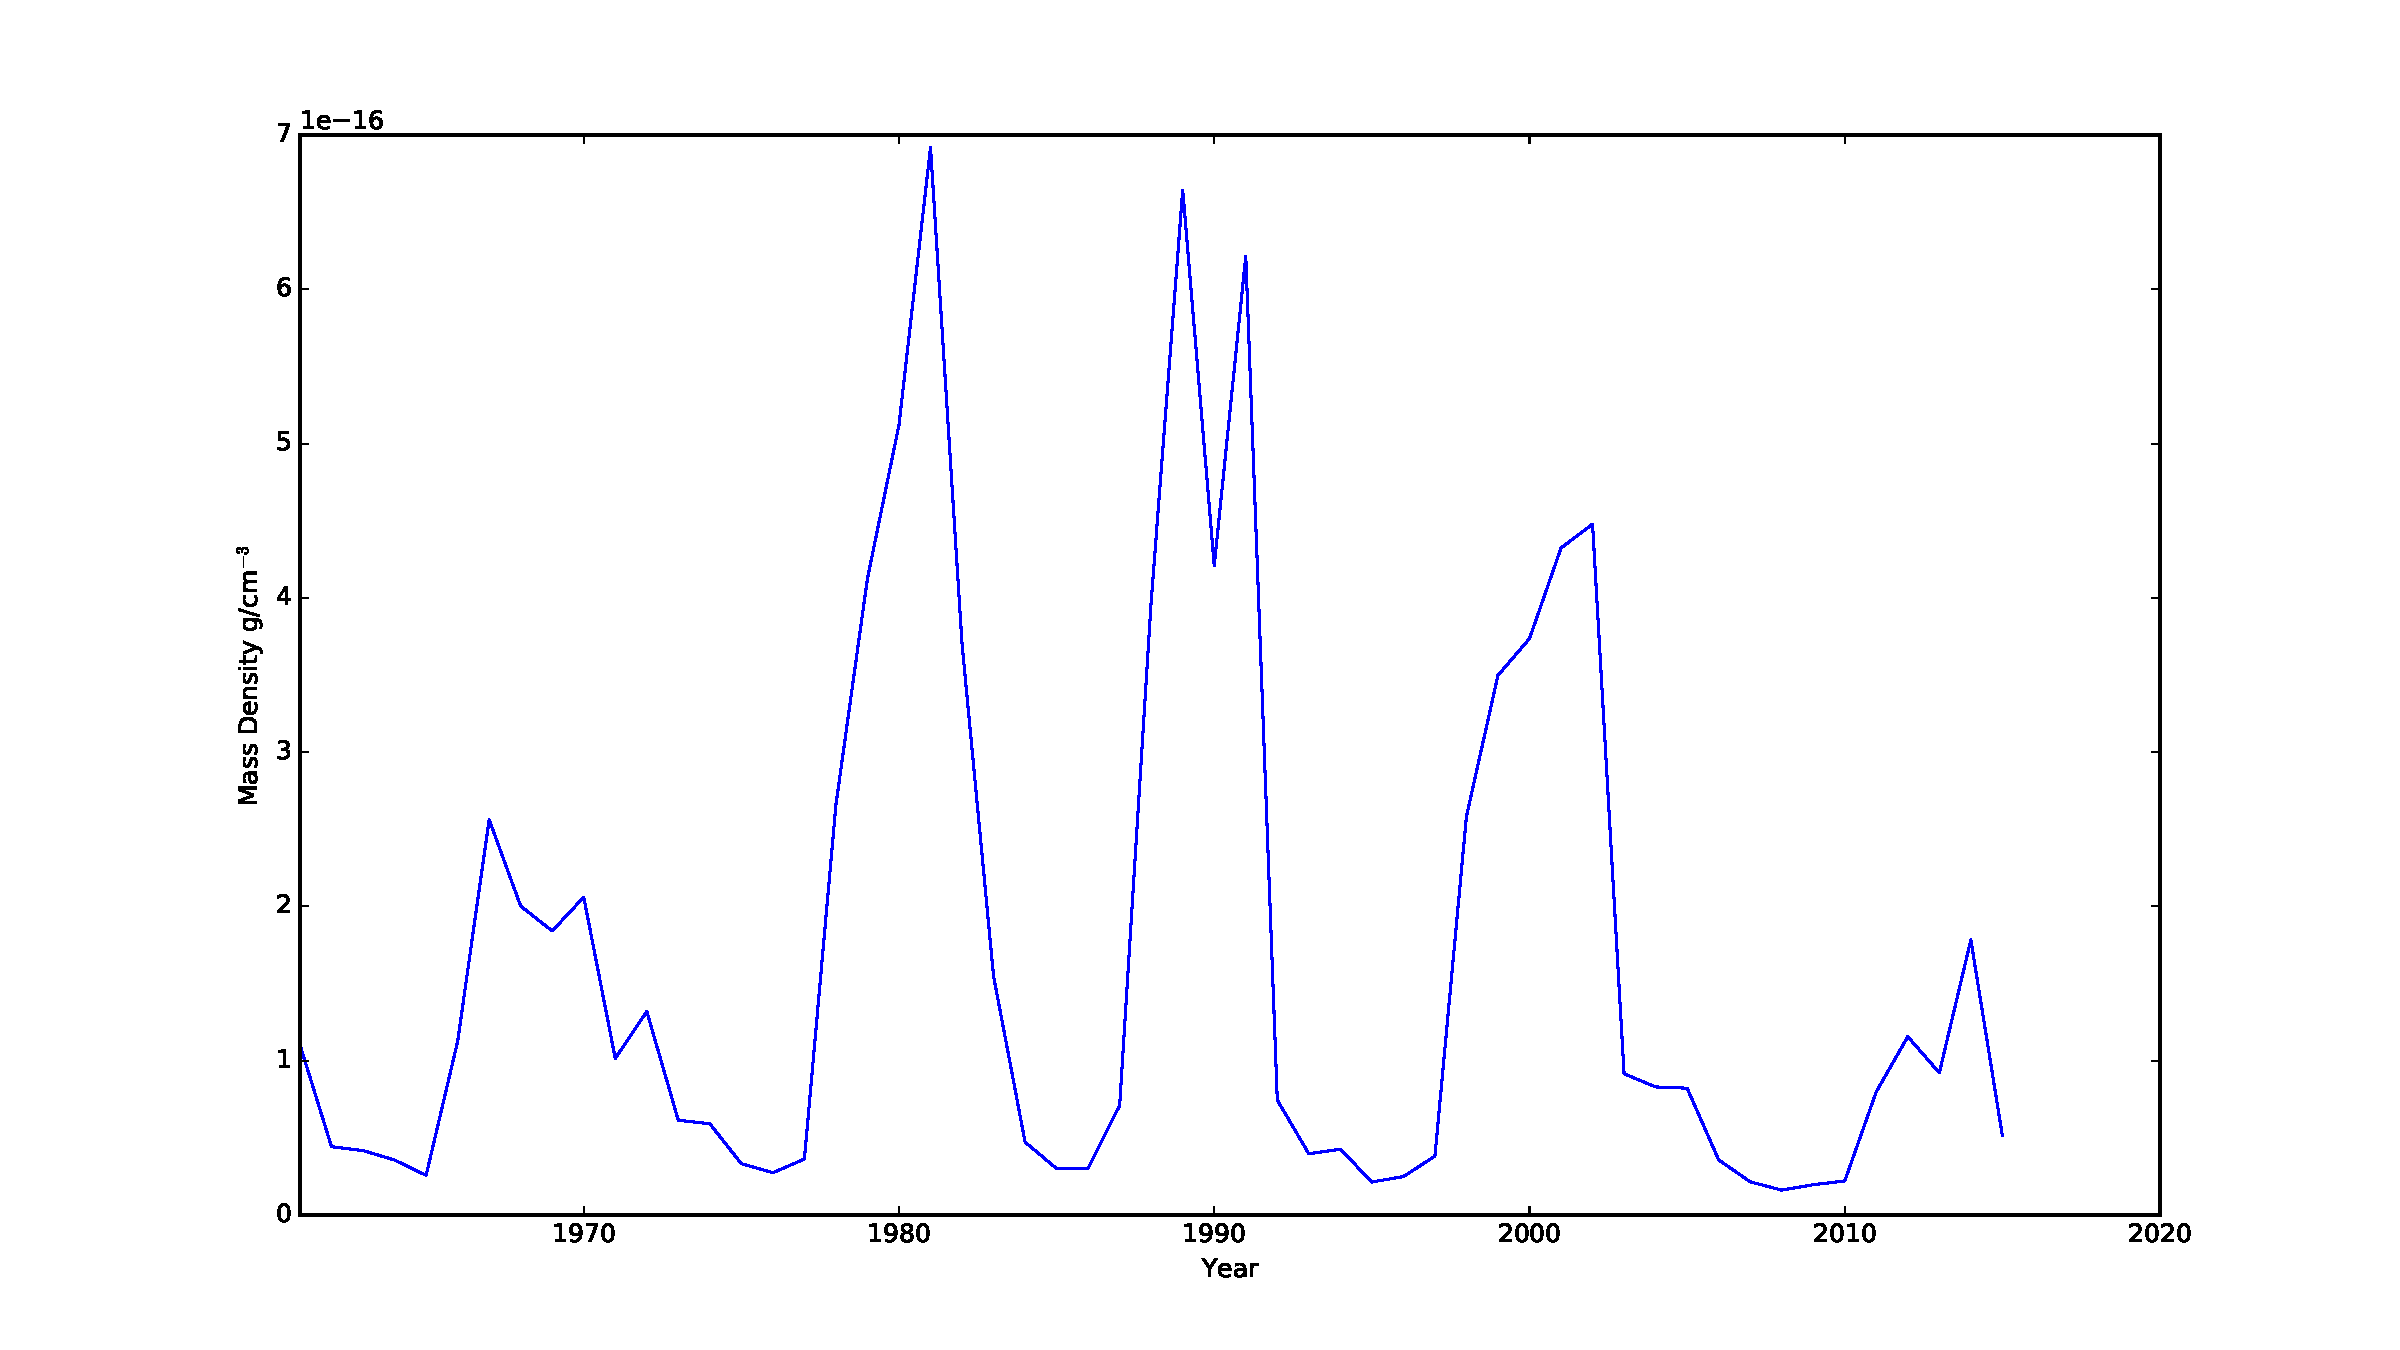
\includegraphics[width=1\textwidth]{MassDensity.pdf}
\caption{Mass density of exosphere from 1961-2015.}
\label{fig:density}
\end{center}
\end{figure}
% Year  Height O, cm-3    Mass density, g/c,-3 Temperature, K
% 2002  550.0  1.445E+07  4.244E-16            983
% 2015  550.0  1.743E+06  5.419E-17            810


\part{Using the NASA NRLMSISE-100 atmosphere model, list the following parameters for today’s date and the HST altitude:}
\begin{enumerate}
\item Atomic oxygen species density
\item Atmosphere mass density
\item Exosphere temperature
\end{enumerate}
\vspace{1em}
The most recent data available is from September 2015. The information for an altitude of 553km is:
\begin{enumerate}
\item Atomic oxygen species density, 1.743E+06 cm$^{-3}$
\item Atmosphere mass density, 5.419E-17 g/cm$^{-3}$
\item Exosphere temperature, 810 K
\end{enumerate}

\part{What role do each of these environmental parameters play in the mission design of your spacecraft?
}

\problem{Orbital Debris and Ballistic Limit Equations (BLE)}
\part{Using eqn 2-3 of the NASA MMOD handbook and Fig 2-4 of the NASA Orbital Debris Engineering Model (both in MMOD folder on SmartSite), determine the critical particle diameter for a Probability of No Penetration (PNP) of 0.877. Assume 1m$^2$ exposed area and
a two-week mission.}

\begin{align*}
  PNP = exp\left[- \sum^{n}_{i=1} \left(F A t\right)_i \right]
\end{align*}
% \eqref{eqn:einstein}
over $n$ spacecraft regions, where $F$ (number/m$^2$-year), of meteoroid and debris impacts that exceed the failure limits (or ballistic limits), the exposed area, A (m$^2$), and duration or time exposed to the MMOD flux, $t$ (year). Plugging in the given values, we have

\begin{align*}
  PNP &= exp\left[- \sum^{n}_{i=1} \left(F A t\right)_i \right] \\
  PNP &= exp\left[- (F A t) \right] \\
  FAt &= ln(\dfrac{1}{PNP})\\
F &= ln(\dfrac{1}{PNP}) \dfrac{1}{At}\\
F &= ln(\dfrac{1}{0.877}) \dfrac{1}{(1)(2*7*24*60*60)}\\
F &= 1.09e-07~[1/m^2/s]
\end{align*}
\noindent Looking at Figure 2-4, we find a diameter of $\approx 0.1$mm.
\part{What would the critical particle diameter be for the same PNP if your spacecraft stayed attached to HST for a second re-boost in 2 years?}
\begin{align*}
F &= ln(\dfrac{1}{PNP}) \dfrac{1}{At}\\
F &= ln(\dfrac{1}{0.877}) \dfrac{1}{(1)(2*365*24*60*60)}\\
F &= 2.08e-09~[1/m^2/s]
\end{align*}
\noindent Looking at Figure 2-4, we find a diameter of $\approx 0.2$mm.

\part{Consider a perpendicular impact of a particle of the size found in part a and another particle with 1mm diameter. Use the Design Equations 4-1 and 4-2 to compute the penetration depth for:}
\begin{enumerate}
\item Silicate particle at 0.5g/cm$^3$ and 23 km/s (micro-meteroid)
\item Steel particle at 7.8 g/cm$^3$ and 7 km/s (orbital debris)
\end{enumerate}
With target materials of:
\begin{enumerate}
\item 6061-T6 Alum
\begin{enumerate}
\item BHN: 95
\item $C_t$: 5.433 km/s
\item Density: 2.7 g/cm$^3$
\end{enumerate}
\item 7075-T6 Alum
\begin{enumerate}
\item BHN: 150
\item $C_t$: 6.350 km/s
\item Density: 2.81 g/cm$^3$
\end{enumerate}
\end{enumerate}

\noindent For $\dfrac{\rho_p}{\rho_t} < 1.5,$
\begin{align*}
P_{\infty} &= 5.24 d^{(19/18)} BHN^{-0.25} \left(\dfrac{\rho_p}{\rho_t}\right)^{0.5} \left(\dfrac{V cos \theta}{C_t}\right)^{2/3}
\end{align*}
For $\dfrac{\rho_p}{\rho_t} \geq 1.5,$
\begin{align*}
P_{\infty} &= 5.24 d^{(19/18)} BHN^{-0.25} \left(\dfrac{\rho_p}{\rho_t}\right)^{2/3} \left(\dfrac{V cos \theta}{C_t}\right)^{2/3}
\end{align*}

\noindent For a silicate particle impacting 6061, we have
\begin{align*}
\dfrac{\rho_p}{\rho_t} &= 0.5/2.7 = 0.19 < 1.5 \\
P_{\infty} &= 5.24 (0.1)^{(19/18)} (95)^{-0.25} \left(\dfrac{0.5}{2.7}\right)^{0.5} \left(\dfrac{23}{5.433}\right)^{2/3} \\
P_{\infty} &= 0.17 cm
\end{align*}

\noindent For a silicate particle impacting 7075, we have
\begin{align*}
\dfrac{\rho_p}{\rho_t} &= 0.5/2.81 = 0.18 < 1.5 \\
P_{\infty} &= 5.24 (0.1)^{(19/18)} (150)^{-0.25} \left(\dfrac{0.5}{2.81}\right)^{0.5} \left(\dfrac{23}{6.350}\right)^{2/3} \\
P_{\infty} &= 0.13 cm
\end{align*}

\noindent For a steel particle impacting 6061, we have
\begin{align*}
\dfrac{\rho_p}{\rho_t} &= 7.8/2.7 = 2.9 > 1.5 \\
P_{\infty} &= 5.24 (0.1)^{(19/18)} (95)^{-0.25} \left(\dfrac{7.8}{2.7}\right)^{2/3} \left(\dfrac{7}{5.433}\right)^{2/3} \\
P_{\infty} &= 0.35 cm
\end{align*}

\noindent For a steel particle impacting 7075, we have
\begin{align*}
\dfrac{\rho_p}{\rho_t} &= 7.8/2.81 = 2.8 > 1.5 \\
P_{\infty} &= 5.24 (0.1)^{(19/18)} (150)^{-0.25} \left(\dfrac{7.8}{2.81}\right)^{2/3} \left(\dfrac{7}{6.350}\right)^{2/3} \\
P_{\infty} &= 0.28 cm
\end{align*}

\part{No protection case: Use Performance Equation 4-6 to estimate the required spacecraft wall thickness to avoid detached spall due to impact of the 1mm particle for the four material cases in part c.}
\part{Compare your answers in part d to equation 4-4.}
\part{Whipple Shield design: For the two 1mm particle compositions/velocities in part c, use equations 4-21 and 4-22 to estimate the bumper and rear-wall thickness required to defeat the threat particles. Assume}
\begin{enumerate}
\item Particles are spherical
\item Bumper standoff = 10.2cm (Fig 4-1)
\item Rear wall: 2219-T87 Alum, 0.5cm thickness
\item Perpendicular velocity impact ($\theta=0$)
\end{enumerate}
\part{Estimate the protection capability limits for your Whipple Shields: Compute the critical projectile performance diameter using equations 4-23, 4-24, and 4-25 for various relative velocities, for two types of spherical particle, one silicate, the other steel. Assume the same parameters as for part f.}

\problem{Acoustic Shielding}
\part{Download and install a sound-level app on your smartphone.}
\part{Measure the sound pressure level (dB) in some noisy environment (home stereo? EFL?).}
\part{Remind yourself: what is the definition of the Decibel, and how is the reference soundpressure level defined?}
\part{Use a Styrofoam cup (or similar) as a payload shroud for your phone. Plug the open end of the shroud with isolation (tissues?). Measure the change in dB sensed by your phone.}
\part{Add some kind of insulation to the inside walls of your payload shroud and repeat part d.}
\part{Discuss results.}

\problem{Numerical Integration Review}
Consider the first-order initial-value problem:
$\dfrac{dy}{dt} = t + y$, $y(0)=0$ with exact solution $y(t) = e^t-t-1$
\part{Program Euler and Runge-Kutta solvers (write your own) and plot the results over a range t=0 to 1.0, with step sizes h=0.01, 0.1, and 0.5. Plot results (y vs t) and compare to the exact solution.}

\begin{figure}[h!]
\begin{center}
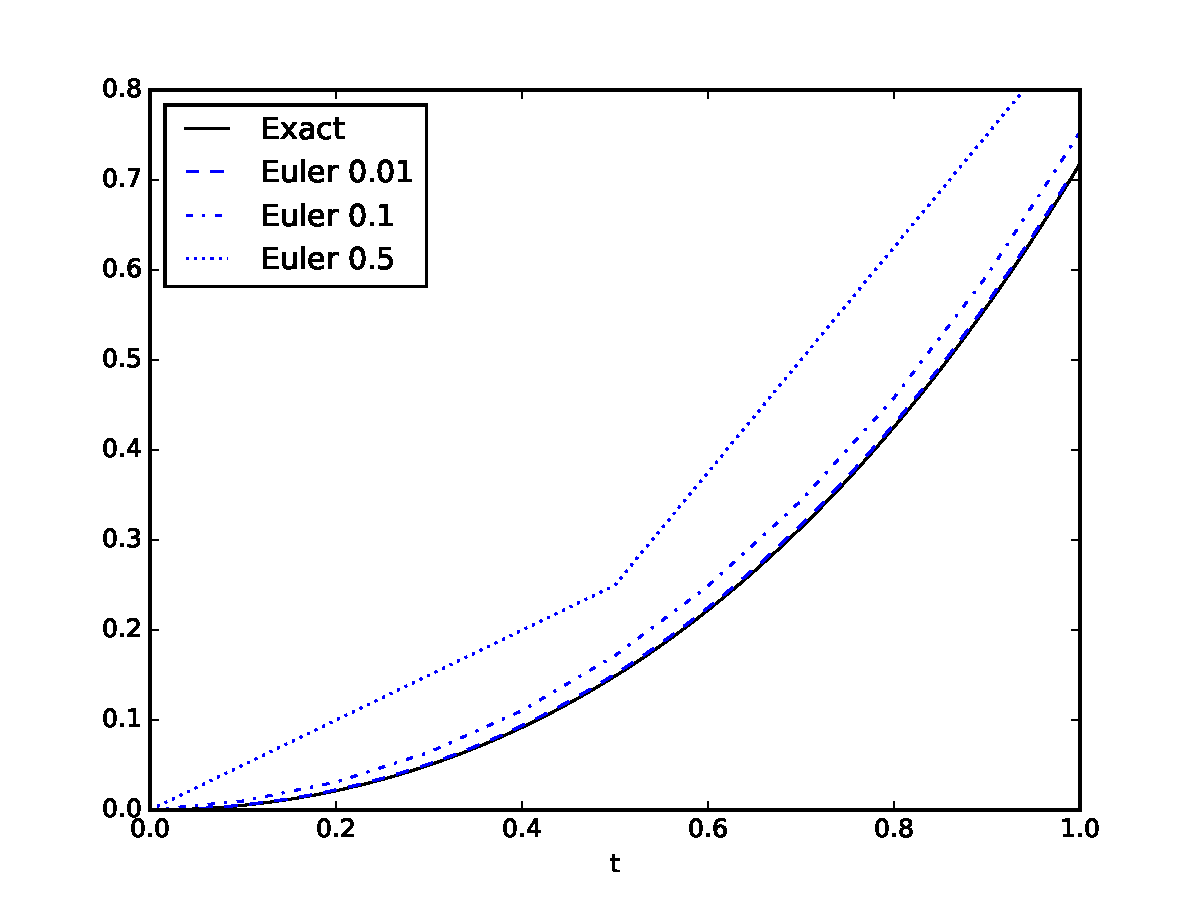
\includegraphics[width=.45\textwidth]{euler.pdf}
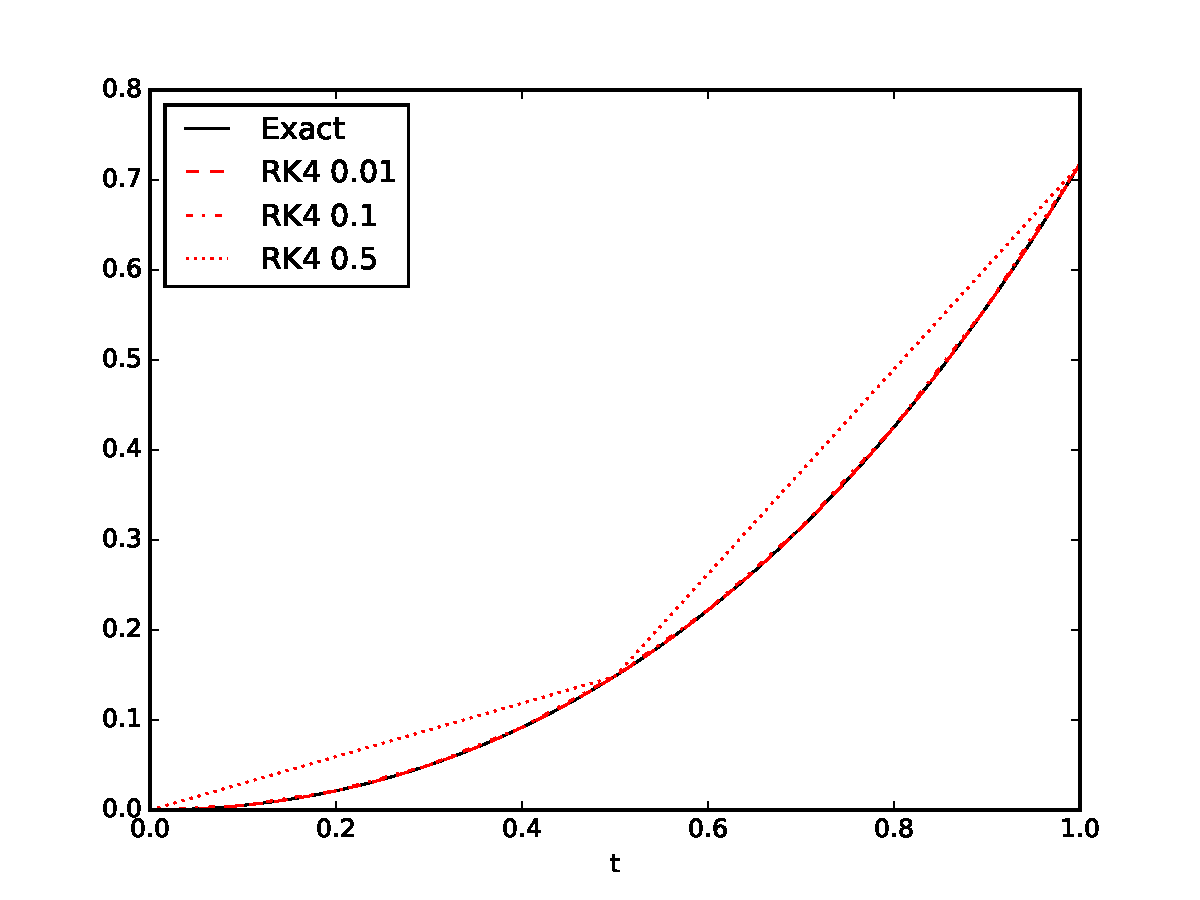
\includegraphics[width=.45\textwidth]{rk4.pdf}
\label{fig:on}
\end{center}
\caption{Results from Euler (left) and RK4 (right) solvers.}
\end{figure}

\part{Repeat step a with library functions for Euler and RK4}
\begin{figure}[h!]
\begin{center}
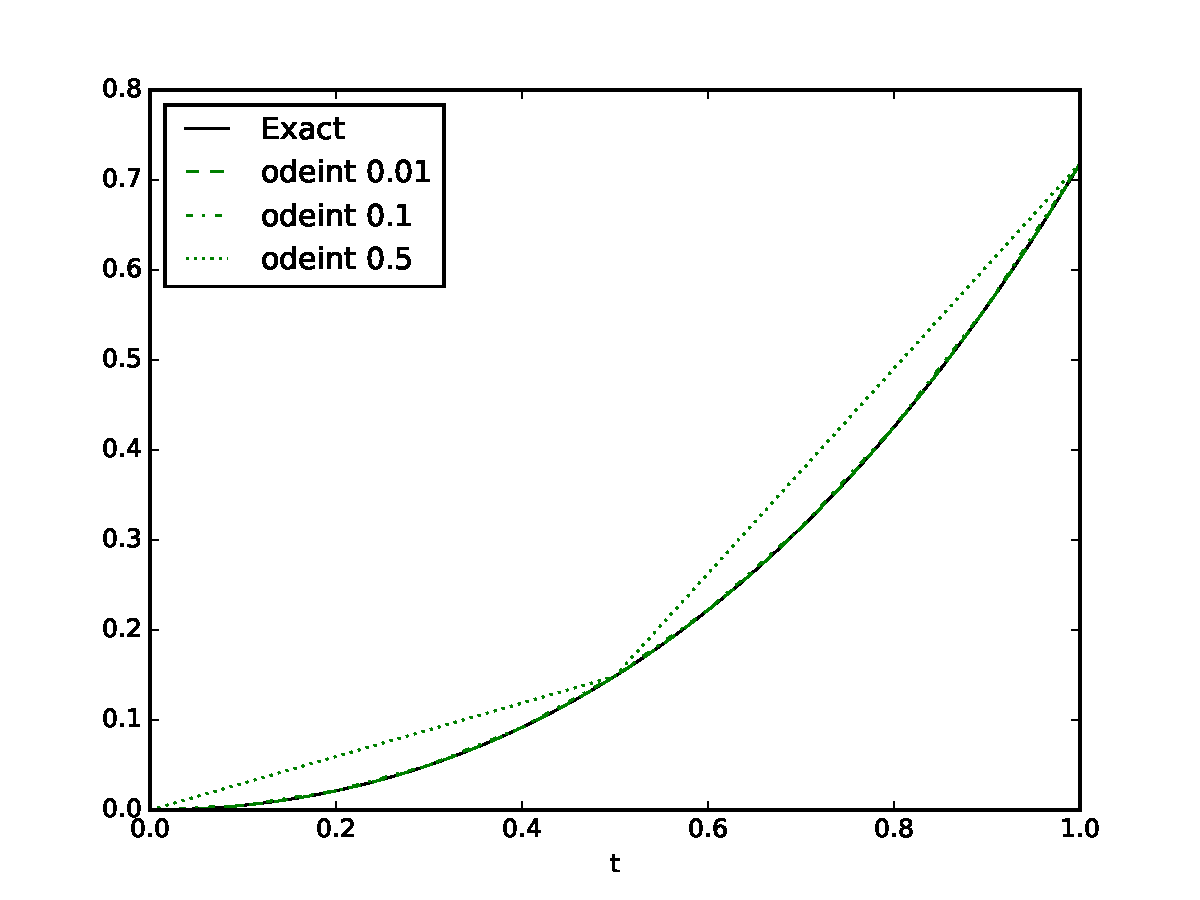
\includegraphics[width=.5\textwidth]{odeint.pdf}
\label{fig:on}
\end{center}
\caption{Results from scipy's RK4 solver.}
\end{figure}

\end{document}
